    \chapter{Arquitetura e Desenho do Sistema}

    \section{Arquitetura Top-Level}
    A arquitetura top-level distingue claramente o produto principal desenvolvido, o \textbf{OmniAI SDK}, da aplicação de validação, a \textbf{OmniAI Gateway}. O SDK contém o domínio comum, os contratos, os adapters, o \textit{dispatcher}, a \textit{pipeline}, os \textit{interceptors}, a DSL de montagem e as abstrações de transporte. A OmniAI Gateway é um POC construído sobre esse SDK: carrega configuração, cria o grafo de componentes, instala os conectores Ktor e expõe endpoints HTTP compatíveis com os contratos estudados.

    \begin{figure}[H]
        \centering
        \begin{tikzpicture}[
            node distance=1.2cm and 1.5cm,
            box/.style={rectangle, draw, rounded corners, align=center, text width=3.8cm, minimum height=1.2cm, inner sep=5pt, thick},
            inner/.style={rectangle, draw, rounded corners, align=center, text width=4.2cm, minimum height=1.0cm, fill=white, inner sep=5pt, thick},
            sdk/.style={rectangle, draw, rounded corners, align=center, text width=4.2cm, minimum height=1.0cm, fill=gray!20, inner sep=5pt, thick},
            group/.style={rectangle, draw, rounded corners, dashed, inner sep=12pt},
            arrow/.style={-Latex, thick}
        ]
            % --- CLIENTES ---
            \node[box] (clients) {Clientes externos\\ex: REST Client, Claude Code};

            % --- OMNIAI GATEWAY (Grupo) ---
            \node[inner, right=1.5cm of clients, yshift=1.2cm] (config) {Configuração do POC \\ \texttt{application.conf}};
            \node[inner, below=0.5cm of config] (ktor) {Gateway Endpoints};
            \node[sdk, below=0.5cm of ktor] (sdk) {OmniAI SDK};

            % O grupo "fit" envolve os blocos internos
            \node[group, fit=(config)(ktor)(sdk), label={[align=center]above:\textbf{OmniAI Gateway POC}}] (gatewayGroup) {};

            % --- LADO DIREITO ---
            \node[box, right=1.5cm of ktor] (providers) {Fornecedores de inferência\\Gemini, Anthropic, OpenAI/Groq};
            \node[box, below=0.8cm of providers] (observability) {Operação local\\Logto, OTel, Prometheus/Grafana};

            % --- LIGAÇÕES ---
            % Entrada do grupo
            \draw[arrow] (clients.east) -- node[above, font=\footnotesize]{} (gatewayGroup.west);

            % Saída do grupo
            \draw[arrow] (gatewayGroup.east) -- node[above, font=\footnotesize]{} (providers.west);
            \draw[arrow] (gatewayGroup.east) -- (observability.west);

        \end{tikzpicture}
        \caption{Arquitetura top-level: POC OmniAI Gateway a instanciar e demonstrar o OmniAI SDK}
        \label{fig:top-level}
    \end{figure}

    \begin{figure}[H]
        \centering
        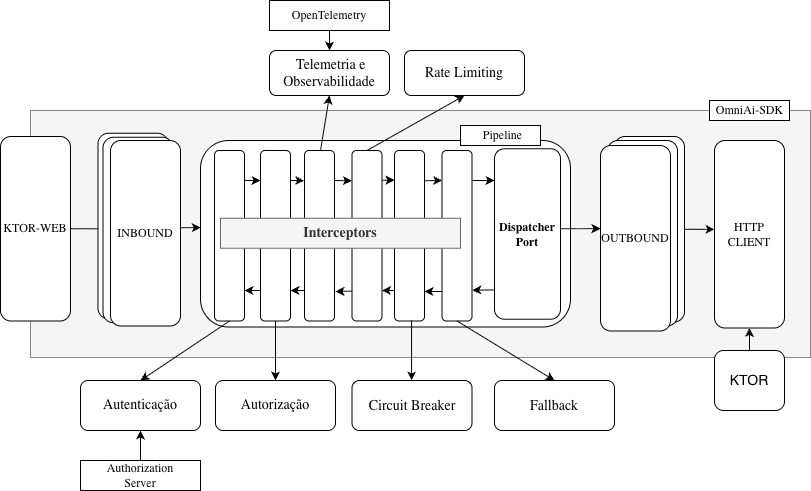
\includegraphics[width=0.95\textwidth]{../images/Arqui}
        \caption{Visão da integração entre Ktor, inbounds, pipeline, interceptors, outbounds e HTTP client no OmniAI SDK}
        \label{fig:arquitet-sdk}
    \end{figure}

    A Figura~\ref{fig:top-level} mostra que o POC não contém a lógica essencial de tradução, despacho ou resiliência. Essa lógica pertence ao SDK e é apenas instanciada pela aplicação final. A Figura~\ref{fig:arquitet-sdk} aproxima a visão interna: um conector HTTP recebe o corpo do pedido, converte-o para um DTO de contrato, invoca um \textit{inbound adapter}, e este chama um \texttt{DispatcherPort}. A partir desse ponto, a execução pode seguir por um dispatcher direto ou por um dispatcher apoiado numa \textit{pipeline}. No final, um \textit{outbound adapter} traduz o pedido comum para o contrato do fornecedor e utiliza um cliente HTTP abstrato para executar a chamada real.

    Esta organização permite que aplicações já compatíveis com APIs existentes possam ser integradas com esforço reduzido. Por exemplo, uma aplicação preparada para a API Anthropic pode alterar o seu \texttt{baseURL} para apontar para a OmniAI Gateway, mantendo o contrato esperado pelo cliente. O mesmo princípio aplica-se a clientes compatíveis com OpenAI e a cenários Gemini suportados pelo POC. A arquitetura foi também pensada para escalamento horizontal: o SDK evita estado global obrigatório, concentra estado transitório no contexto do pedido e define portas para substituir stores em memória por backends partilhados quando a Gateway é executada em múltiplas instâncias.

    \section{Arquitetura Hexagonal (Ports \& Adapters)}
    A Arquitetura Hexagonal foi escolhida para separar a lógica de domínio dos detalhes de transporte, dos contratos externos e das bibliotecas concretas. A formulação original de Cockburn descreve a aplicação no centro e os mecanismos externos ligados através de portas e adapters \cite{cockburn_hexagonal}. Esta abordagem é particularmente adequada a uma Gateway de IA, porque o sistema é dominado por integrações: clientes externos, APIs de fornecedores, servidores de autorização, telemetria e mecanismos de transporte.

    Uma alternativa seria uma arquitetura em camadas tradicional, com controladores, serviços e repositórios. Essa opção seria simples no início, mas tenderia a concentrar traduções de contratos, chamadas HTTP e regras operacionais no mesmo serviço de aplicação. Outra alternativa seria decompor cedo a solução em vários serviços independentes. Essa abordagem poderia escalar equipas e deploys, mas introduziria complexidade operacional excessiva para um SDK cujo objetivo principal é ser reutilizável dentro de diferentes aplicações. A opção hexagonal oferece um compromisso mais adequado: mantém uma estrutura modular e testável sem obrigar a transformar cada responsabilidade num serviço remoto. No contexto de gateways, esta separação também acompanha o padrão de API Gateway como camada de integração e política transversal \cite{api_gateway_design,ai_gateway_pattern,karl_ai_gateway}.

    \subsection{Contracts}
    Os módulos \texttt{contracts:openai}, \texttt{contracts:anthropic} e \texttt{contracts:gemini} modelam os formatos de pedido, resposta e eventos de cada fornecedor. Estes contratos são DTOs no sentido em que representam dados transportados na fronteira do sistema, mas não são apenas DTOs genéricos. São chamados \textit{contracts} porque codificam uma compatibilidade externa concreta: nomes de campos, estruturas JSON, eventos de \textit{streaming}, campos opcionais, formatos de erro e convenções específicas de cada API.

    Esta distinção é importante. Um DTO interno poderia ser livremente alterado sem impacto externo; um contrato compatível com OpenAI, Anthropic ou Gemini precisa de respeitar o formato que clientes e fornecedores esperam. Ao isolar estes contratos em módulos próprios, o SDK evita que detalhes como \texttt{tool\_calls}, \texttt{content\_block\_delta} ou \texttt{functionDeclarations} se espalhem pelo domínio comum.

    \subsection{Inbounds}
    Os \textit{inbound adapters} recebem pedidos no formato do cliente e traduzem-nos para \texttt{CommonRequest}. Cada inbound implementa a porta \texttt{InboundPort} e recebe um \texttt{DispatcherPort}, não uma implementação concreta de pipeline ou de fornecedor. Além disso, cada inbound usa uma implementação de \texttt{InboundTranslator}, responsável por converter o objeto de entrada para domínio e por converter a resposta comum de volta para o contrato do cliente.

    Esta decisão evita que o inbound exponha diretamente uma Web API. O SDK fornece adapters que trabalham sobre objetos de transferência, e a exposição HTTP fica noutro adapter, como o \texttt{gateway-ktor-server}. Assim, um servidor Ktor, uma função serverless, um handler Express ou outro mecanismo de entrada podem chamar o mesmo inbound desde que consigam construir o DTO esperado. Esta separação reduz a dependência do domínio e dos inbounds face a bibliotecas HTTP externas.

    \subsection{Outbounds}
    Os \textit{outbound adapters} fazem o caminho inverso: recebem um \texttt{CommonRequest}, traduzem-no para o contrato do fornecedor real e executam a chamada externa. Cada outbound implementa \texttt{OutboundPort}, identifica \texttt{provider}, \texttt{model} e \texttt{key}, e delega a tradução num \texttt{OutboundTranslator}. A implementação atual inclui outbounds para OpenAI, Anthropic e Gemini.

    Ao contrário dos inbounds, os outbounds precisam de comunicar com serviços externos. Por isso recebem uma implementação de \texttt{HttpTransportClient}. A implementação fornecida pelo SDK é baseada em Ktor, mas a porta permite substituir o transporte por outro cliente HTTP, por um mock em testes, por um cliente instrumentado ou por uma implementação específica de plataforma. Esta inversão de dependência é o que permite testar adapters sem depender de chamadas reais e evoluir o runtime sem reescrever o domínio.

    \subsection{Dispatcher}
    O \texttt{DispatcherPort} é a porta chamada pelos inbounds para executar um \texttt{CommonRequest}. A sua responsabilidade não é, por si só, conter inteligência de roteamento; é despachar o pedido para uma estratégia de execução. No SDK é fornecida uma implementação simples, criada por \texttt{routingDispatcherFactory}, que procura o outbound cujo \texttt{provider} e \texttt{model} correspondem aos campos do pedido e envia a chamada para esse adapter.

    Como se trata de uma interface, a arquitetura permite outras implementações com objetivos diferentes. Um consumidor do SDK pode fornecer um dispatcher direto, um dispatcher com seleção por custo, um dispatcher que consulta políticas externas ou um dispatcher que aplica regras mais complexas. A \textit{pipeline} fornecida pelo SDK é ela própria encaixada através de um adapter, \texttt{PipelineBackedDispatcher}, preservando a ideia de que os inbounds dependem apenas de \texttt{DispatcherPort}.

    \section{Ecossistema do SDK}
    O SDK está organizado como um projeto Gradle multi-módulo. Os módulos principais incluem \texttt{core}, \texttt{contracts}, \texttt{inbound}, \texttt{outbound}, \texttt{interceptors}, \texttt{mcp-broker}, \texttt{dispatcher}, \texttt{gateway-client}, \texttt{gateway-ktor-server} e \texttt{contracts:ktor-http}. Esta divisão permite evoluir cada área com responsabilidades claras: domínio e portas em \texttt{core}, contratos externos em \texttt{contracts}, adapters de entrada e saída em módulos próprios, preocupações transversais em \texttt{interceptors}, montagem declarativa em \texttt{gateway-client} e exposição HTTP/Ktor em \texttt{gateway-ktor-server}.

    O módulo \texttt{contracts:ktor-http} fornece a abstração de transporte \texttt{HttpTransportClient} e a implementação \texttt{KtorHttpTransportClient}. Esta camada encapsula chamadas HTTP, SSE, serialização, metadados de resposta, erros de rede e erros de parsing. Ao colocá-la atrás de uma interface, os outbounds não ficam presos a uma implementação específica de cliente HTTP.

    O módulo \texttt{gateway-client} disponibiliza uma DSL para montar uma Gateway. A aplicação consumidora pode declarar outbounds, interceptors, autenticação, autorização e modo de execução. A DSL permite escolher entre \texttt{useNativePipeline}, que monta a pipeline e o dispatcher padrão, e \texttt{useCustomDispatcher}, que permite substituir totalmente a estratégia de execução. Esta flexibilidade é essencial para um SDK: o POC usa a montagem nativa, mas outro consumidor pode querer um dispatcher próprio.

    A aplicação \texttt{OmniAiGateway} foi desenvolvida como POC de validação do SDK. O uso de \textit{composite build} do Gradle, através de \texttt{includeBuild("../OmniAi-SDK")} \cite{gradle_composite_builds}, não pretende simular a forma final de consumo em produção. A sua função foi acelerar o desenvolvimento do projeto final, permitindo compilar SDK e POC em conjunto, testar alterações imediatamente e evitar o ciclo pesado de publicar uma versão do SDK, atualizar dependências do POC e voltar a compilar. Numa distribuição real, a expectativa é que o SDK seja consumido como dependência versionada, nomeadamente via Maven para JVM e via NPM para Node.js/TypeScript.

